% !TEX root = ../ac_paper.tex

\section{Classical Search Algorithms} \label{sec:search}

\begin{algorithm}
	\caption{Greedy Search Algorithm}\label{alg:bfs}
	\begin{algorithmic}
		\State $Q \gets P_0$ \Comment{Initialize the prioriy queue of presentations with $P_0$.}
		\State $S \gets P_0$ \Comment{Initialize the set of seen presentations with $P_0$.}

		\While{$\text{len}(S) < 10^6$} \Comment{While the number of distinct states is less than $10^6$.}
		\State $P \gets Q[0]$ \Comment{Pop the top element of the heap.}
		\For{$A \in \text{AC Moves}$}
		\State $PA \gets A \cdot P$ \Comment{Act on $P$ by $A$.}
		\If{PA is trivial}
		\Return{True}
		\Else{ $PA \notin S$}
		\State $S \gets PA$
		\State $Q \gets PA$ \Comment{Insert $PA$ to $Q$ with priority.}

		\EndIf
		\EndFor
		\EndWhile
	\end{algorithmic}
\end{algorithm}

% Sketch of the section: We use search algorithm to get a baseline on results. We call it breadth-first search. It is able to solve less than half of the presentations we considered. We will use these presentations to generate dataset for each of the techniques used in the next two sections: for embeddings, we generate text dataset, for reinforcement learning, these states are the initial states of a Markov Decision Process. 

%\fixme{Made search space finite. Perhaps this could be discussed in the previous section. Justify the BFS name.}

In this section, we introduce a greedy search algorithm, referenced as \autoref{alg:bfs}, which bears resemblance to the A* search algorithm within the context of graph theory. The algorithm searches the space of all balanced presentations for a path that connects an initial presentation $P_0$ to a trivial presentation.
$P_0$ is initially placed into a priority queue $Q$ and a set $S$. The priority queue is ordered by a tuple $(k, l)$ where $k$ is the total length of a presentation and $l$ is the path length between a state and $P_0$. The algorithm iteratively selects the top element from the priority queue and applies all possible AC moves to it to generate new states. If a state has not been seen before, the algorithm adds it to both $Q$ and $S$. This process is continued until the algorithm finds a trivial presentation, deeming the search successful, or if it has seen a million distinct states. 
%Note that the paths found by our greedy search algorithm depend on the particular order in which AC moves are applied. 
\newline

We place a cutoff of a million states to make the search process feasible within a practical timeframe. We will call a presentation ``GS-easy" if the greedy search algorithm successfully finds a path that trivializes the presentation; otherwise, we will call it ``GS-hard". The distributions of ``GS-easy" and ``GS-hard" presentations as functions of $n$ and lengths of the presentations of the Miller-Schupp series is given in \autoref{fig:miller_schupp_statistics}. 
\footnote{\fixme{Is it better to use 'GS-easy'/GS-hard or GS-solved/GS-unsolved? Fix the figure accordingly, i.e. replaced 'solved' and 'unsolved' by 'GS-solved' and 'GS-unsolved'.}}
\footnote{\fixme{One issue with the bar chart is that it does not give precise numbers for solved and unsolved presentations. If we need to provide those explicit numbers, we can use heatmaps instead.}}
Note that the number of unsolved presentations increases monotonically with $n$, but not with the total length of the presentation. This indicates that $n$ as compared to the length of the presentation is a better metric to measure the hardness of a presentation. 
All presentations with total length up to 13 are solved. 
There are a total of six unsolved presentations at length 14, four of which are AC-equivalent to $\AK(3)$. The other two presentations are as follows. 
\[
\angles{x, y \mid x^{-1} y^2 x = y^{3} , x = y x^2 y^{\pm 1} x^{-2}}
\]
We checked that these presentations are not AC-equivalent to $\AK(3)$ by any sequence of AC moves that allows the length of each relator to increase upto 20.

\fixme{What is the maximum length each relator is allowed to take in my GS?}

\fixme{Compare the performance with an ordinary BFS algorithm. I set it up to run on Feb 23 with SLURM ID: 34869100. Compare it also with a GS/BFS algorithm that applies the usual AC moves. 34869254 has GS with original AC moves and 34869256 has BFS with original AC moves.}

Update: there was an issue with 34869254. I submitted a new run 34943081 after fixing the issue. 

Can we say anything about the structure of graph of AC presentations? It is not a tree. (What's the argument for it?) 

%It is listed as example 1 on page 3 of \cite{MMS}.
%I have checked whether we can reduce the length of these examples with max length = 20.

%\fixme{Compare with Table 2 of Panteleev-Ushakov.
%They seem to have a lot more examples with $n=2$ that they could not resolve.}


%The number of BFS-hard examples increases as a function of $n$.
%(See \autoref{fig:hist_vs_n}.)
%The distributions of BFS-easy and BFS-hard as a function of the total length of a presentation are also given in \autoref{fig:hist_vs_length}.


\begin{figure}
	\centering
	\begin{subfigure}[b]{0.5\textwidth}
		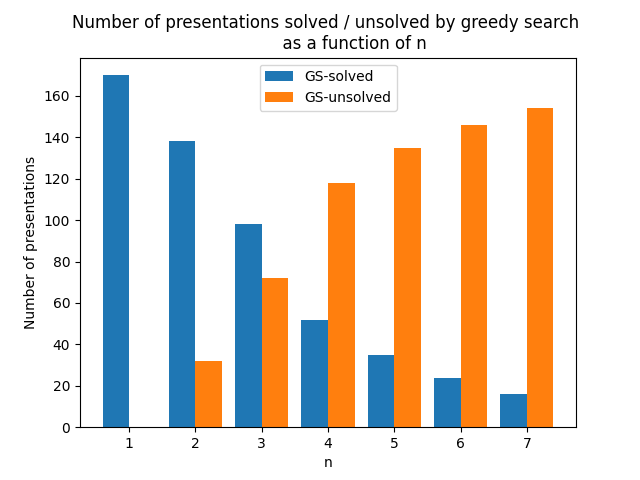
\includegraphics[width=\textwidth]{fig/hist_vs_n.png}
		\caption{Distribution versus $n$}
		\label{fig:hist_vs_n}
	\end{subfigure}%
	%add desired spacing between images, e. g. ~, \quad, \qquad etc.
	%(or a blank line to force the subfigure onto a new line)
	\begin{subfigure}[b]{0.5\textwidth}
		\centering
		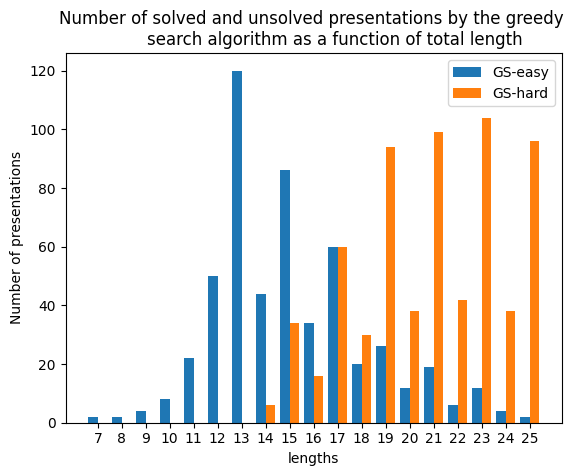
\includegraphics[width=1.1\textwidth]{fig/hist_vs_lengths.png}
		\caption{Distribution versus total length}
		\label{fig:hist_vs_length}
	\end{subfigure}
	\caption{Number of GS-solved and GS-unsolved presentations as functions of $n$ and total length of the presentation. A presentation is GS-solved (GS-unsolved) if the greedy search algorithm in  \autoref{alg:bfs} could (could not) trivialize the presentation. The subfigure on the left (right) shows the number of GS-solved and GS-unsolved presentations in the Miller-Schupp series as a function of $n$ (the total length of the presentation). The number of GS-unsolved presentations increases monotonically with $n$. } \label{fig:miller_schupp_statistics}
	
I don't think I need to check BFS for all cases of $n$. Already at $n=1$, GS is able to solve all presentations while BFS is not. This is proof that GS is superior to BFS.



As for original AC moves vs our AC moves, BFS with original AC moves also seems to be not able to solve many $n=1$ presentations. So the only comparison of interest here is GS with original AC moves vs GS with our AC moves. Since GS sorts the priority queue by the length of the presentation, I will not be surprised if GS with our AC moves does slightly better. The run of GS with original AC moves,  34869254, should be done in another day or so.


\fixme{Perhaps all $n=1$ examples will be solved by finding paths using the original AC moves, i.e. the pattern will be more obvious that way.}

\fixme{What's the longest length that a presentation obtains before it is trivialized? This is especially a question about $n=1$. In $n=1$, do lengths ever go above the original length?}

\fixme{Be careful about full simplify vs simplify in presenting results. }

\end{figure}